%!TEX root = ../main.tex

\section{Introduction}
\label{section:cfgnn-introduction}
Advances in machine learning (ML) have led to breakthroughs in several areas of science and engineering,  ranging from computer vision, to natural language processing, to conversational assistants. 
Parallel to the increased performance of ML systems, there is an increasing call for the ``understandability'' of ML models ~\citep{goebel-2018-explainable}. 
Understanding \emph{why} an ML model returns a certain output in response to a given input is important for a variety of reasons such as model debugging, aiding decison-making, or fulfilling legal requirements \citep{gdpr}. 
Having certified methods for interpreting ML predictions will help enable their use across a variety of applications~\citep{miller-2017-explanations}.



Explainable artificial intelligence (XAI) refers to the set of techniques ``\textit{focused on exposing complex AI models to humans in a systematic and interpretable manner}''~\citep{samekexplainable}. A large body of work on XAI has emerged in recent years~\citep{guidotti-2018-survey,bodria2021benchmarking}. Counterfactual explanations are used to explain predictions of individual instances in the form: ``If X had been different, Y would not have occurred''~\citep{stepin2021survey,karimi_model-agnostic_2019,schut_generating_2021}. 
Counterfactual explanations are based on counterfactual examples: modified versions of the input sample that result in an alternative output (i.e., prediction). 
If the proposed modifications are also \emph{actionable}, this is referred to as achieving recourse \citep{ustun_actionable_2019,karimi2020survey}. 

To motivate our problem, consider an ML application for computational biology: drug discovery is a task that involves generating new molecules that can be used for medicinal purposes \citep{stokes_deep_2020,xie2021mars}. 
Given a candidate molecule, a GNN can predict if this molecule has a certain property that would make it effective in treating a particular disease \citep{wieder_compact_2020,guo2021fewshot,nguyen2020metalearning}.
%If the GNN predicts it does not have this desirable property, counterfactual explanations can help identify the minimal change required in order for the molecule to have the desirable property. 
%This could help us not only generate a new molecule that has this property, but also understand the molecular structures that contribute to this property.
If the GNN predicts it does not have this desirable property, counterfactual explanations can help identify the minimal change required such that the molecule is predicted to have this property. 
This could help not only inform the design of a new molecule that has this property, but also understand the molecular structures that contribute to this property.


Although GNNs have shown state-of-the-art results on tasks involving graph data \citep{zitnik_modeling_2018,deac_drug-drug_2019}, existing methods for explaining the predictions of GNNs have primarily focused on generating subgraphs that are relevant for a particular prediction~\citep{yuan2020explainability,baldassarre_explainability_2019,duval2021graphsvx,lin_causal_2021,luo_parameterized_2020,pope_explainability_2019,schlichtkrull_interpreting_2020,vu2020pgmexplainer,ying_gnnexplainer_2019,yuan_subgraph_2021}. 
However, \emph{none of these methods are able to identify the minimal subgraph automatically} -- they all require the user to specify the size of the subgraph, $S$, in advance. 
We show that even if we adapt existing methods to the counterfactual explanation problem, and try varying values for $S$, such methods are not able to produce valid, accurate counterfactual explanations, and are therefore not well-suited to solve the counterfactual explanation problem. 
To address this gap, we propose CF-GNNExplainer, a method for generating counterfactual explanations for GNNs. 

Similar to other counterfactual methods for tabular or image data proposed in the literature~\citep{verma2020counterfactual, karimi2020survey}, CF-GNNExplainer works by perturbing input data at the instance-level. 
Unlike previous methods, CF-GNNExplainer can generate counterfactual explanations for graph data. 
In particular, our method iteratively removes edges from the original adjacency matrix based on matrix sparsification techniques, keeping track of the perturbation that leads to a change in prediction, and returning the perturbation with the smallest change w.r.t.\ the number of edges. 

\begin{figure}[t]
    \centering
    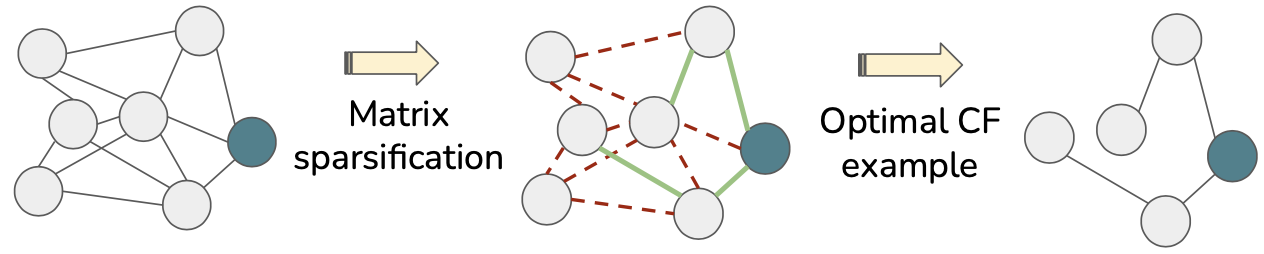
\includegraphics[width=\columnwidth]{04-research-cfgnn/images/visual.png}
    \caption{Intuition of counterfactual example generation by CF-GNNExplainer.}
    \label{fig:visual}
\end{figure}

\pagebreak

We evaluate CF-GNNExplainer on three public datasets for GNN explanations and measure its effectiveness using four metrics: fidelity, explanation size, sparsity, and accuracy. We find that CF-GNNExplainer is able to generate counterfactual examples with at least 94\% accuracy, while removing fewer than 3 edges on average. 
We make the following contributions:
\begin{enumerate}[(1)]
    \item We formalize the problem of generating counterfactual explanations for GNNs (Section~\ref{section:problem-formulation}). 
    \item We propose CF-GNNExplainer, a novel method for explaining predictions from GNNs (Section~\ref{section:cfgnn-method}). 
    \item We propose an experimental setup for holistically evaluating counterfactual explanations for GNNs (Section~\ref{section:cfgnn-experimental-setup}).
\end{enumerate}   



